% =====================================================================
\section{Phase 1: making the data}\label{sec:p1}
% =====================================================================

\textbf{Goal.} Produce realistic observations of a known law, so that every later phase can be graded against
a truth it is not allowed to see.

\textbf{What happens.} \fn{data/generate_diffusion.py} simulates $u_t = 0.1\,u_{xx}$ on $x\in[0,1]$,
$t\in[0,1]$ with the explicit finite-difference scheme (61 grid points $\times$ 800 time steps), starting
from the double hump $\sin(\pi x) + 0.5\sin(3\pi x)$ with both ends held at zero. From the full field it
saves three files:

\begin{center}
\small
\begin{tabular}{@{}lp{11.5cm}@{}}
\toprule
\fn{full.npz} & the entire clean field (800$\times$61). For grading and plots only. \\
\fn{sparse.npz} & a noise-free random 10\% of grid points (4880 points). For ablations of sparsity alone. \\
\fn{noisy.npz} & \textbf{400 random points with Gaussian noise} (std = 5\% of the field's std, $\approx0.0116$).
                 \textbf{The only file the discovery system may see}, and it uses only its $x,t,u$ columns. \\
\bottomrule
\end{tabular}
\end{center}

\begin{figure}[!htb]
\centering
% flowchart 'p1' -- shared by project_guide.tex and submission_report.tex
\begin{tikzpicture}[node distance=4mm and 6mm]
  \node[fnw=cData] (main) {main\\{\normalfont\tiny generate\_diffusion.py}};
  \node[fnw=cData, below=of main] (cfg) {load_config\\{\normalfont\tiny read config.yaml}};
  \node[fnw=cData, below=of cfg] (full) {build_full_field\\{\normalfont\tiny x, t grids; call the solver}};
  \node[fnw=cData, right=of full] (ic) {initial_condition\\{\normalfont\tiny one sine, two sines, or a Gaussian bump}};
  \node[fnw=cData, below=of ic] (fd) {solve_diffusion_fd\\{\normalfont\tiny explicit FTCS steps, $D=0.1$}};
  \node[fnw=cData, below=of full, yshift=-12mm] (flat) {flatten_field\\{\normalfont\tiny grid $\to$ (x, t, u) rows}};
  \node[fnw=cData, below=of flat] (samp) {make_sparse_and_noisy\\{\normalfont\tiny 10\% subsample; 400 pts + 5\% noise}};
  \node[io, below=of samp] (files) {full.npz\quad sparse.npz\quad noisy.npz};
  \node[fnw=cData, right=of files, xshift=4mm] (test) {tests/test_diffusion_data\\{\normalfont\tiny sanity checks + verification plot}};
  \draw[flow] (main) -- (cfg); \draw[flow] (cfg) -- (full);
  \draw[flow] (full) -- (ic); \draw[flow] (ic) -- (fd); \draw[flow] (fd) |- (flat);
  \draw[flow] (full) -- (flat); \draw[flow] (flat) -- (samp); \draw[flow] (samp) -- (files);
  \draw[dflow] (files) -- (test);
\end{tikzpicture}

\pkglegend
\caption{Phase~1 function flow: configuration $\to$ simulation $\to$ sampling $\to$ files $\to$ checks.}
\label{fig:p1}
\end{figure}

\begin{figure}[!htb]
\centering
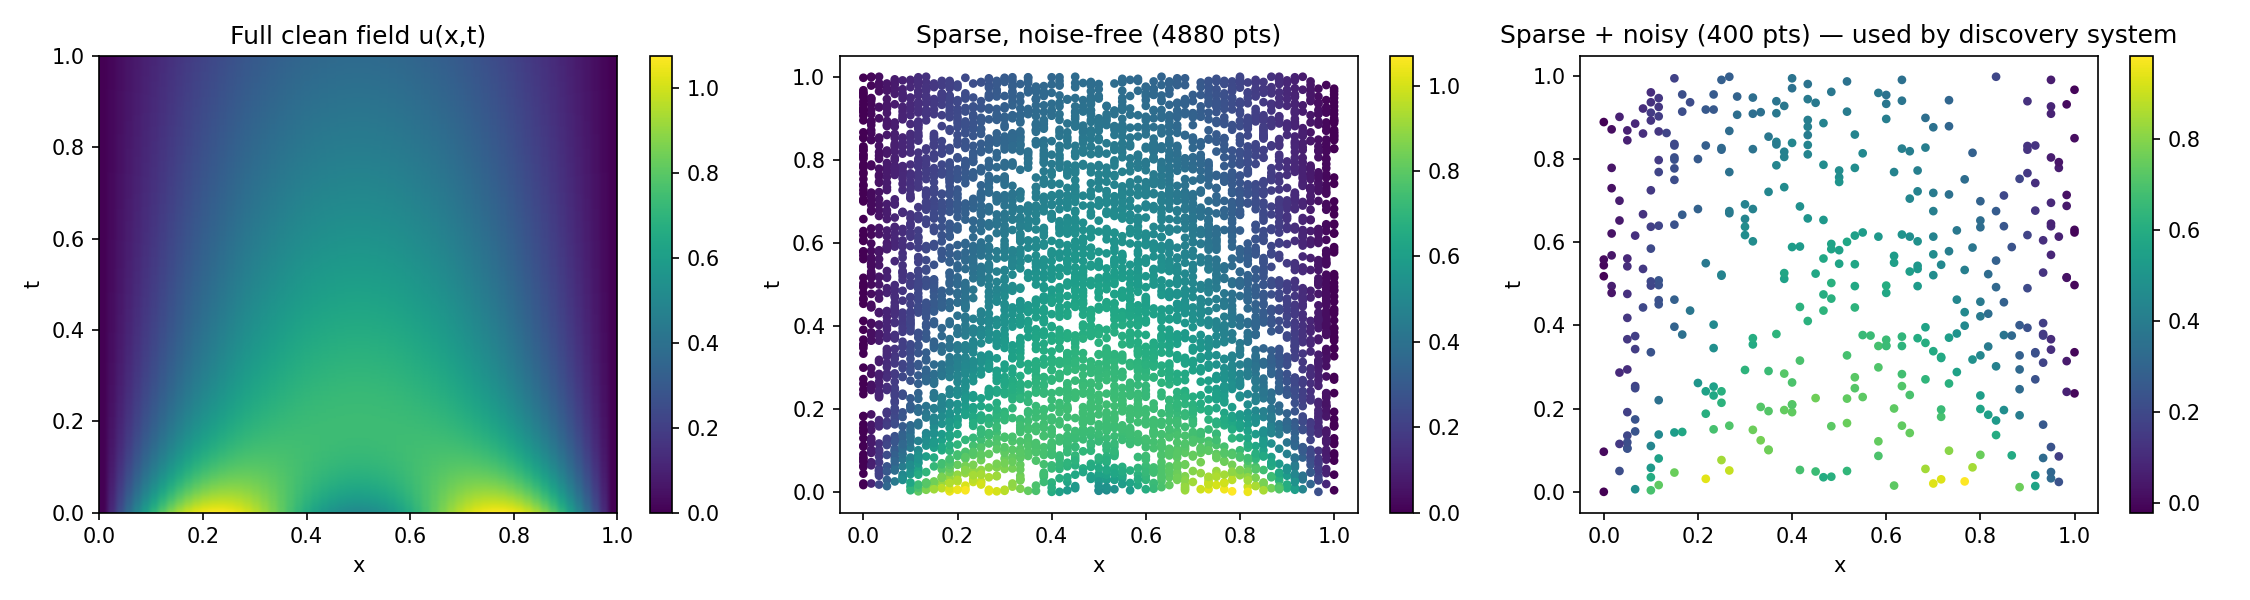
\includegraphics[width=0.95\textwidth]{data/generated/verification_plot.png}
\caption{Phase~1 verification plot (from the project's results): the clean field (left), the sparse sample, and
the 400 noisy points the system is allowed to see. The double hump decays and merges into one broad hump,
because the faster-wiggling mode $\sin(3\pi x)$ decays 9 times faster than $\sin(\pi x)$.}
\end{figure}

\begin{lesson}[: the eigenfunction trap]
The first version started from a single $\sin(\pi x)$. That turned out to be undiscoverable: for this profile
$u_{xx}=-\pi^2u$ exactly, so ``$D\,u_{xx}$'' and ``$-D\pi^2u$'' are the same signal and no method can separate
them. The two-mode start mixes two different curvatures and breaks the tie. The single-mode option is kept in
the code as a documented cautionary example, and Phase~7's adversarial suite re-tests it (case A13).
\end{lesson}

% =====================================================================
\section{Phase 2: equation discovery by sparse regression}\label{sec:p2}
% =====================================================================

\textbf{Goal.} Recover $u_t \approx D\,u_{xx}$ from data alone using SINDy (Section~\ref{sec:sindy}), and
report honestly where it works and where it does not.

\textbf{How it works.} For clean data (already a grid), take finite differences directly. For scattered data,
first reconstruct a grid by linear interpolation (41$\times$150 nodes for 4880 sparse points, but only
13$\times$25 for 400 noisy points), optionally smooth it with a Gaussian filter, then difference. Build the
8-column library and run STLSQ with threshold 0.05.

\begin{figure}[!htb]
\centering
% flowchart 'p2' -- used by docs/Report.tex
\begin{tikzpicture}[node distance=4mm and 7mm]
  \node[fnw=cExp] (main) {02_equation_discovery.main};
  \node[fnw=cExp, below=of main] (case) {run_case\\{\normalfont\tiny once per dataset: clean, sparse, noisy$\times$2}};
  \node[dec=cEqd, below=7mm of case] (q) {on a grid\\already?};
  \node[fnw=cEqd, right=of q, xshift=6mm] (scat) {discover_from_scatter};
  \node[fnw=cEqd, below=of scat] (rec) {reconstruct_grid\\{\normalfont\tiny scipy griddata, linear}};
  \node[fnw=cEqd, below=of rec] (sm) {smooth_grid\\{\normalfont\tiny Gaussian denoising (noisy only)}};
  \node[fnw=cEqd, below=34mm of q] (grid) {discover_from_grid};
  \node[fnw=cEqd, below=of grid] (fields) {_fields_from_grid};
  \node[fnw=cEqd, below=of fields] (fdd) {finite_diff_derivatives\\{\normalfont\tiny central differences (np.gradient)}};
  \node[fnw=cEqd, right=of fdd, xshift=6mm] (specs) {parse_term_specs\\{\normalfont\tiny config lists $\to$ term tuples}};
  \node[fnw=cEqd, below=of fdd] (lib) {build_library + term_label\\{\normalfont\tiny the 8 columns of $\Theta$}};
  \node[fnw=cEqd, below=of lib] (sindy) {run_sindy};
  \node[fnw=cEqd, right=of sindy, xshift=6mm] (stlsq) {stlsq\\{\normalfont\tiny fit, zero small, refit, repeat}};
  \node[fnw=cEqd, below=of sindy] (str) {equation_to_string};
  \node[fnw=cEqd, below=of str] (gt) {evaluate_against_ground_truth\\{\normalfont\tiny grading only, after discovery}};
  \node[fnw=cEqd, right=of str, xshift=6mm] (comp) {evaluate_competing_hypotheses\\{\normalfont\tiny diffusion-only vs advection-only fit}};
  \node[fnw=cEqd, below=of comp] (restr) {fit_restricted\\{\normalfont\tiny least squares on fixed terms}};
  \node[io, below=of gt] (out) {phase2\_discovery\_report.json, table, plot};
  \draw[flow] (main) -- (case); \draw[flow] (case) -- (q);
  \draw[flow] (q) -- node[note, above]{no} (scat);
  \draw[flow] (q) -- node[note, right]{yes} (grid);
  \draw[flow] (scat) -- (rec); \draw[flow] (rec) -- (sm); \draw[flow] (sm) |- (grid);
  \draw[flow] (grid) -- (fields); \draw[flow] (fields) -- (fdd); \draw[flow] (fdd) -- (lib);
  \draw[flow] (specs) |- (lib);
  \draw[flow] (lib) -- (sindy); \draw[flow, <->] (sindy) -- node[note, above]{loop} (stlsq);
  \draw[flow] (sindy) -- (str); \draw[flow] (str) -- (gt); \draw[flow] (gt) -- (out);
  \draw[dflow] (case.east) -| ([xshift=4mm]comp.east) -- (comp.east);
  \draw[flow] (comp) -- (restr);
\end{tikzpicture}

\pkglegend
\caption{Phase~2 function flow. Scattered data is first put on a grid; then derivatives, library, sparse
regression. The competing-hypothesis check (right) fits each single-term law separately.}
\label{fig:p2}
\end{figure}

\textbf{Results.}
\begin{center}
\small
\begin{tabular}{@{}lllc@{}}
\toprule
\textbf{Data} & \textbf{Discovered equation} & $\hat D$ (error) & \textbf{Right terms?} \\ \midrule
Clean  & $u_t = 0.1009\,u_{xx}$ & 0.1009 (0.9\%) & yes \\
Sparse & $u_t = 0.1013\,u_{xx}$ & 0.1013 (1.3\%) & yes \\
Noisy, no smoothing & $0.50 - 3.42u + 4.15u^2 + \ldots$ (5 terms) & -- & no \\
Noisy, smoothed & $0.55u + 0.20u_{xx} - 0.51u^2 + \ldots$ (5 terms) & -- & no \\
\bottomrule
\end{tabular}
\end{center}
On noisy data the free 8-term search fails. But the evidence is still there: fitting single-term laws gives
diffusion $R^2 = 0.79$ ($\hat D = 0.107$) while advection has \emph{negative} $R^2$ (worse than predicting the
mean) on every dataset. So advection is correctly disfavoured even when the unrestricted search is confused.

\begin{figure}[!htb]
\centering
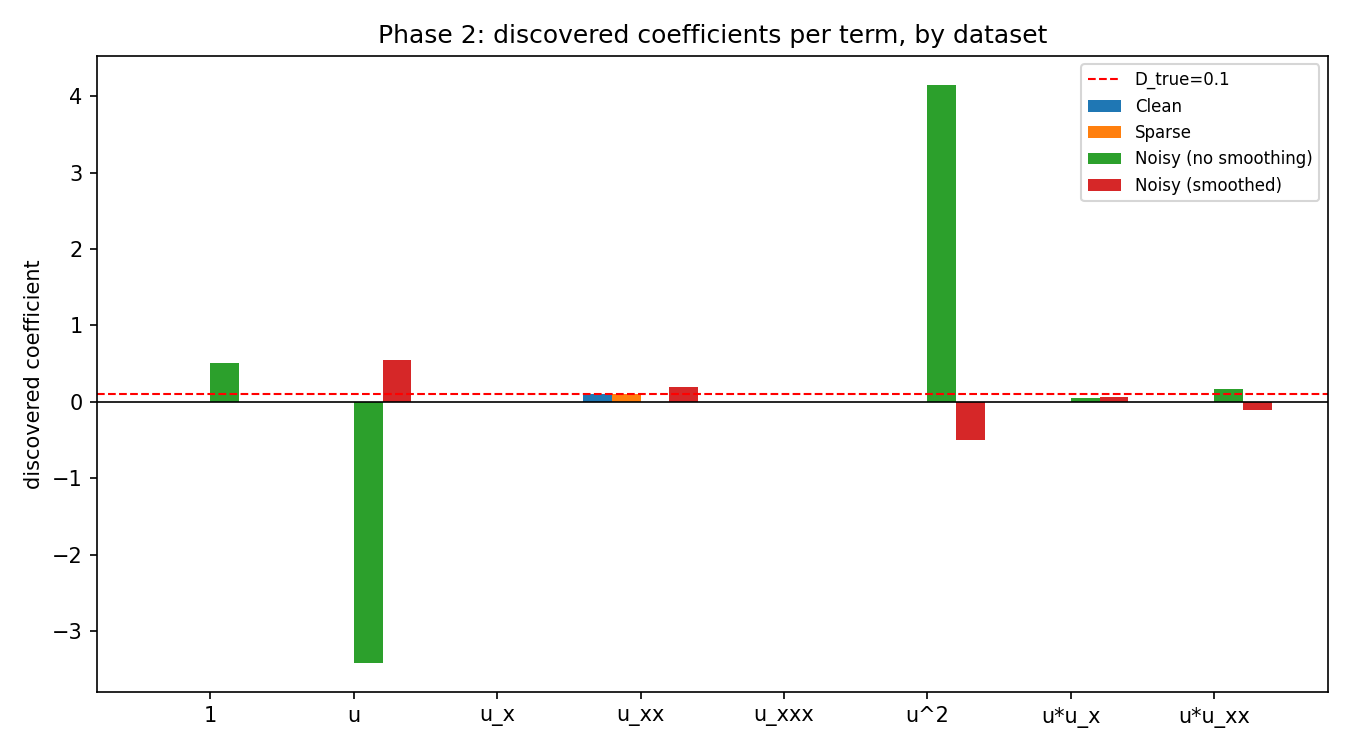
\includegraphics[width=0.88\textwidth]{results/equations/phase2_coefficients.png}
\caption{Phase~2 coefficients found by STLSQ for each run (from \fn{results/equations/}). Clean and sparse data
keep only $u_{xx}$; noisy data scatters weight over spurious terms.}
\end{figure}

\begin{lesson}[: a good fit is not the right law]
Noisy SINDy produced equations with small residuals and wrong terms. Differentiating noisy data amplifies the
noise (Section~\ref{sec:background}), and regression then explains noise with extra terms. This motivates
Phase~3: test hypotheses with a method that never differentiates the data.
\end{lesson}

% =====================================================================
\section{Phase 3: physics-informed neural networks}\label{sec:p3}
% =====================================================================

\textbf{Goal.} Build one reusable PINN (Section~\ref{sec:pinn}) and use it three ways: forward (known $D$),
inverse (estimate $D$), and hypothesis validation (diffusion vs.\ advection).

\textbf{How it works.} The network \fn{PINN} maps $(x,t)\mapsto u$ with four tanh layers of 64 units. The
\emph{only} thing that changes between hypotheses is the residual function, looked up in
\fn{RESIDUAL_REGISTRY} (diffusion, advection, reaction--diffusion). All derivatives come from autograd
(\fn{compute_derivatives}). Training draws 2000 collocation points, 200 boundary and 200 initial points, runs
3000 Adam steps then 300 L-BFGS iterations, and finally scores the result against fixed thresholds.

\begin{figure}[!htb]
\centering
% flowchart 'p3' -- used by docs/Report.tex
\begin{tikzpicture}[node distance=3.6mm and 6mm]
  % left column: experiment set-up
  \node[fnw=cExp] (main) {04_inverse_pinn.main\\{\normalfont\tiny (03 forward, 05 hypothesis vs hypothesis)}};
  \node[fnw=cPinn, below=of main] (load) {load_observational_data\\{\normalfont\tiny noisy.npz: x, t, u only}};
  \node[fnw=cPinn, below=of load] (pts) {make_collocation_points\\make_bc_points, make_ic_points};
  \node[fnw=cPinn, below=of pts] (tens) {data_dict_to_tensors\\filter_by_time};
  \node[fnw=cPinn, below=of tens] (inv) {run_inverse_pinn\\{\normalfont\tiny (run\_forward\_pinn: D fixed)}};
  \node[fnw=cPinn, below=of inv] (bt) {build_and_train};
  \node[fnw=cPinn, below=of bt] (net) {PINN\\{\normalfont\tiny 2 $\to$ 64$\times$4 tanh $\to$ 1}};
  \node[fnw=cPinn, below=of net] (mp) {make_params\\{\normalfont\tiny D as trainable tensor}};
  \node[fnw=cPinn, below=of mp] (tr) {PINNTrainer.train\\{\normalfont\tiny Adam 3000 $\to$ L-BFGS 300}};
  % right column: one loss evaluation
  \node[fnw=cPinn, right=of tr, xshift=10mm, yshift=46mm] (cl) {PINNTrainer.compute_losses};
  \node[fnw=cPinn, below=of cl] (cd) {compute_derivatives\\{\normalfont\tiny exact derivatives by autograd}};
  \node[fnw=cPinn, below=of cd] (res) {residual_fn\\{\normalfont\tiny from the residual registry}};
  \node[fnw=cPinn, below=of res] (loss) {data_loss, physics_loss\\bc_loss, ic_loss};
  \node[fnw=cPinn, below=of loss] (tot) {total_loss\\{\normalfont\tiny weighted sum (all weights 1)}};
  \begin{scope}[on background layer]
    \node[pkgbox=cPinn, fit=(cl)(cd)(res)(loss)(tot), label={[pkglabel=cPinn]above:one optimisation step}] (box) {};
  \end{scope}
  % scoring
  \node[fnw=cVal, below=of tr] (phys) {evaluate_physics_residual\\{\normalfont\tiny residual on a fresh grid}};
  \node[fnw=cVal, below=of phys] (ood) {split_by_time + prediction_error\\{\normalfont\tiny in-distribution vs $t>0.7$}};
  \node[fnw=cVal, below=of ood] (score) {build_validation_result\\{\normalfont\tiny thresholds $\to$ supported / rejected}};
  \foreach \a/\b in {main/load,load/pts,pts/tens,tens/inv,inv/bt,bt/net,net/mp,mp/tr,tr/phys,phys/ood,ood/score}
    \draw[flow] (\a) -- (\b);
  \draw[flow] (tr.east) -- (box.west |- tr.east) node[note, above, pos=0.45]{each step};
  \draw[flow] (cl) -- (cd); \draw[flow] (cd) -- (res); \draw[flow] (res) -- (loss); \draw[flow] (loss) -- (tot);
\end{tikzpicture}

\pkglegend
\caption{Phase~3 function flow. Left: an experiment builds tensors, creates the network and trains it. Right: what
happens inside every optimisation step. Bottom: scoring with fixed thresholds.}
\label{fig:p3}
\end{figure}

\textbf{Results.}
\begin{itemize}
  \item \textbf{Forward} ($D=0.1$ known): the PINN's prediction differs from the clean field by RMSE
        $0.000727$, even though it was trained on data with $\approx0.0116$ noise. The physics term denoises.
  \item \textbf{Inverse} ($D$ unknown, started at 0.2): $\hat D = 0.09989$, a 0.11\% error. $D$ slides from 0.2
        to 0.1 within about 1500 Adam steps and stays there.
  \item \textbf{Validation}, both trained on $t\le0.7$ only with their parameter trainable:
\end{itemize}
\begin{center}
\small
\begin{tabular}{@{}lllllll@{}}
\toprule
\textbf{Hypothesis} & \textbf{Status} & \textbf{Data loss} & \textbf{Physics} & \textbf{IC loss} & \textbf{In-dist.\ RMSE} & \textbf{OOD RMSE} \\ \midrule
H1 diffusion & supported & 0.00013 & 0.00008 & 0.000001 & 0.00078 & 0.00115 \\
H2 advection & rejected  & 0.03775 & 0.00499 & 0.02515  & 0.20033 & 0.33145 \\
\bottomrule
\end{tabular}
\end{center}
Diffusion wins on every metric by 30--290$\times$. Advection simply cannot turn a decaying double hump into
anything consistent with the data: its IC loss alone is 25{,}000 times worse.

\begin{figure}[!htb]
\centering
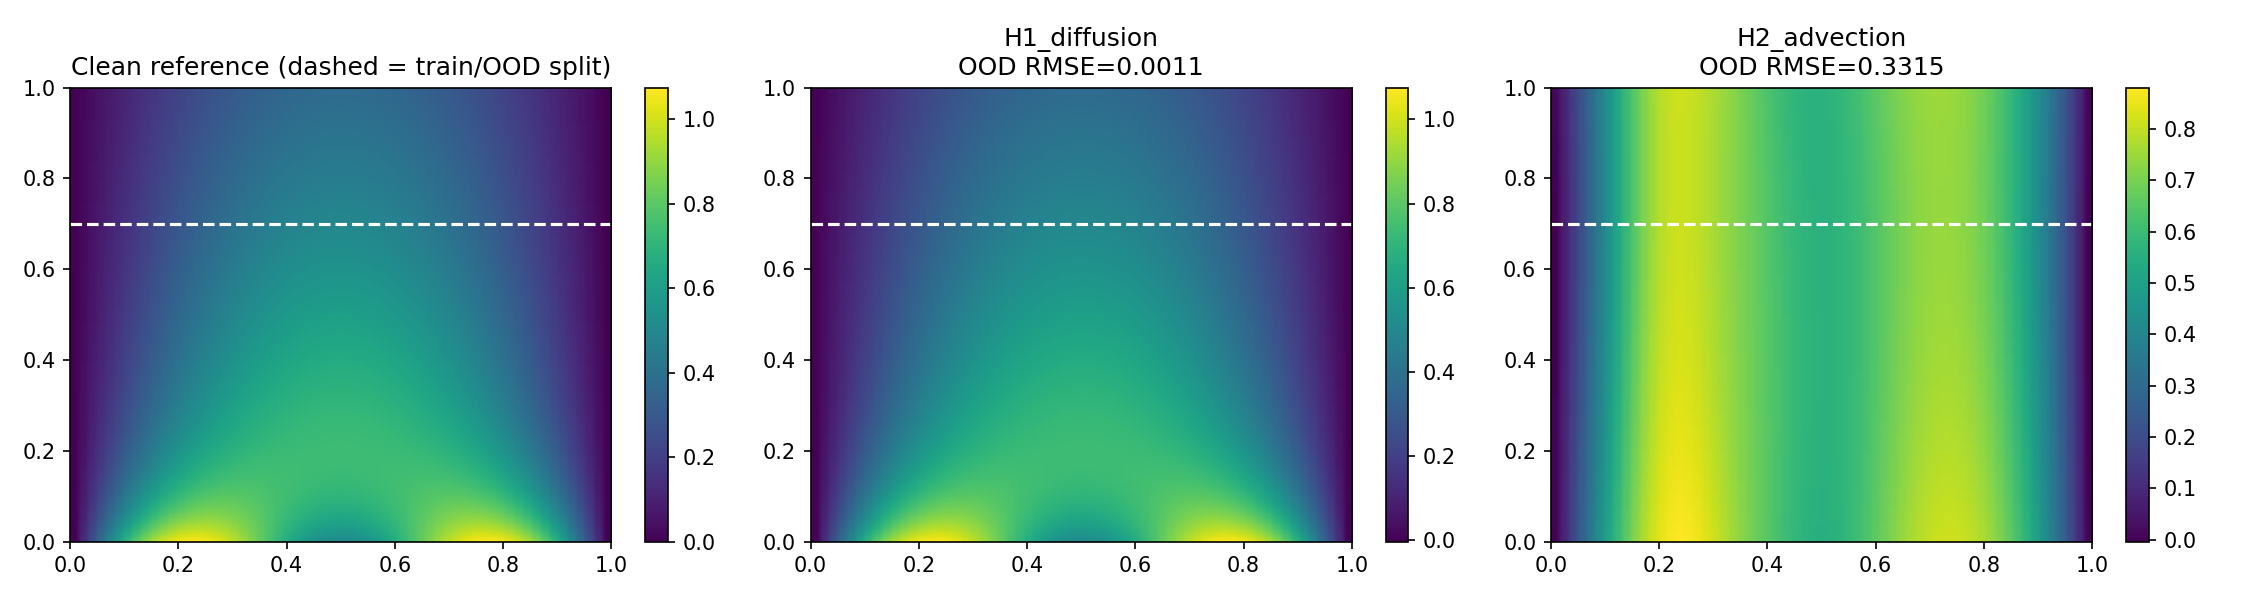
\includegraphics[width=0.92\textwidth]{results/pinn/phase3_ood_comparison.png}
\caption{Phase~3 hypothesis validation (from \fn{results/pinn/}). Training used only $t\le0.7$ (dashed line).
Diffusion reproduces the field on both sides of the split; advection converges to a wrong, roughly static
pattern.}
\end{figure}

\begin{caution}[: an audit note added in Phase 6]
The Phase~3 accept/reject rule included one check against the clean truth field. Training never used it, but a
decision did. Re-checking showed no outcome depended on it (H2 also fails its data and IC losses). Phase~6
removed the issue: from then on, decisions use only held-out \emph{noisy} observations.
\end{caution}
